\documentclass[../main.tex]{subfiles}


\begin{document}
\subsection{VM cliente Linux}\label{sec:cliente_vmlinux}
\begin{table}[htbp]
  \centering
  \begin{tabular}{rl}
    
    hostname:&Node02\\
    Sistema Operativo:&Centos 8\\
  \end{tabular}
\end{table}

\subsection{Tarjeta de red}\label{sec:ctr}
\begin{table}[htbp]
  \centering
  \begin{tabular}{rl}
    
    IP:&$192.168.100.28/24$\\
    Puerta de Enlace&$192.168.100.1$\\
    Broadcast:&$192.168.100.255$\\
    DNS:&$192.168.100.119\ 8.8.8.8$\\
    Dominio AC:&SRV\\
  \end{tabular}
\end{table}


\subsection{Configuracion}\label{sec:cliente_conf}

\subsubsection{Linux}\label{sec:cliente_linux}

\paragraph{Añadir dominio}
\begin{enumerate}
  \item Se debe modificar el archivo \texttt{/etc/hosts} añadiendo
        el dominio del servidor.
        \begin{listing}[H]
\begin{minted}{linux-config}
192.168.100.119 Node03.srv.nis srv.nis Node03 srv
\end{minted}
\label{list:hosts}
\caption{Modificación del archivo /etc/hosts}
\end{listing}
\end{enumerate}

\paragraph{NIS}
\begin{enumerate}
  \item Instalar los paquetes necesarios.
        \begin{listing}
\begin{minted}{shell-session}
$ dnf -y install ypbind rpcbind oddjob-mkhomedir
\end{minted}
\end{listing}

  \item Configurar el dominio del NIS

        Usar \texttt{ypdomainname} como usuario adiministrativo.
        \begin{listing}[H]
\begin{minted}{shell-session}
$ ypdomainname srv.world
\end{minted}
\end{listing}
        Añadir el dominio a \texttt{/etc/sysconfig/network}
        \begin{listing}[H]
\begin{minted}{bash}
$ echo "NISDOMAIN=srv.world" >> /etc/sysconfig/network
\end{minted}
\label{list:sysnetwork}
\caption{Modificación del archivo /etc/sysconfig/network}
\end{listing}
        Añadir el servidor al la configuracion de NIS \texttt{/etc/yp.conf}
        \begin{listing}[H]
\begin{minted}{linux-config}
# [domain (NIS domain) server (NIS server)]
domain srv.nis server Node03.srv.nis
\end{minted}
\label{list:yp}
\caption{Modificación del archivo /etc/yp.conf}
\end{listing}

  \item Configurar el metodo de autenticacion del cliente

        Añadir NIS como metodo de autenticacion

        \begin{listing}[H]
\begin{minted}{shell-session}
authselect select nis --force
profile "nis" was selected.
The following nsswitch maps are overwritten by the profile:
- aliases
- automount
- ethers
- group
- hosts
- initgroups
- netgroup
- networks
- passwd
- protocols
- publickey
- rpc
- services
- shadow

Make sure that NIS service is configured and enabled. See NIS documentation for more information.
\end{minted}
\end{listing}

  \item Añadir la caracteristica para crear directorio de home al
        primer inicio de sesion

        \begin{listing}[H]
\begin{minted}{shell-session}
$ authselect enable-feature with-mkhomedir
\end{minted}
\end{listing}

  \item Habilitar nis en SELinux (o desactivar SELinux si no es indispensable).

        \begin{listing}[H]
\begin{minted}{shell-session}
$ setsebool -P nis_enabled on
\end{minted}
\end{listing}

  \item Habilitar el servicio en systemd

        \begin{listing}[H]
\begin{minted}{shell-session}
$ systemctl enable --now rpcbind ypbind nis-domainname oddjobd
\end{minted}
\end{listing}

  \item Probar la correcta cofiguracion del cliente

        Confirma si el enlazador tiene comunicacion con el servidor NIS
        \begin{listing}[H]
\begin{minted}{shell-session}
$ ypwhich
\end{minted}
\end{listing}
  \item Si todo sale bien debe aparecer el servidor en el dominio
        \begin{listing}[H]
\begin{minted}{shell-session}
Node03.src.nis
\end{minted}
\end{listing}
  \item Cambiar contraseña de NIS (Se proporcionara un
        script bash para automatizar este proceso)

        \begin{listing}[H]
\begin{minted}{shell-session}
$ yppasswd
\end{minted}
\end{listing}

\end{enumerate}


\paragraph{NFS}
\begin{enumerate}
  \item Instalar los paquetes necesarios para NFS

        \begin{listing}[H]
\begin{minted}{shell-session}
$ dnf -y install nfs-utils
\end{minted}
\end{listing}
  \item Configurar el dominio del servidor NFS en el
        archivo \texttt{/etc/idmapd.conf}
        \begin{listing}[H]
\begin{minted}{linux-config}
# linea 5 donde esta el dominio por defecto poner el del servidor
Domain = srv.nis
\end{minted}
\label{list:idmap}
\caption{Modificación del archivo /etc/idmapd.conf}
\end{listing}

  \item Probar que hay acceso al servidor nfs

        Montar la carpeta del servidor NFS

        \begin{listing}[H]
\begin{minted}{shell-session}
$ mount -t nfs Node03.srv.nis:/home /home
\end{minted}
\end{listing}

        Si todo sale bien correr el siguiente comando que mostara que
        efectivamente esta operativa la particion del tipo nfs4

        \begin{listing}[H]
\begin{minted}{linux-config}
df -hT /home
S.ficheros           Tipo Tamaño Usados  Disp Uso% Montado en
Node03.srv.nis:/home nfs4    19G   1.3G   17G   8% /home
\end{minted}
\end{listing}

  \item Añadir la particion al fstab, esto montara la carpeta una vez
        que se inicia el sistema

        Modificar el archivo \texttt{/etc/fstab}
        \begin{listing}[H]
\begin{minted}{linux-config}
# Añadir al final del archivo
Node03.srv.nis:/home/ /home               nfs     defaults        0 0
\end{minted}
\label{list:fstab}
\caption{Modificación del archivo /etc/fstab}
\end{listing}

  \item Añadir el montaje dinamico\footnote{En caso de una caida
        del servidor este volvera a montar cada vez que se
        quiera acceder al directorio asignado al NFS}

        Instalar AutoFS

        \begin{listing}[H]
\begin{minted}{shell-session}
$ dnf -y install autoFS
\end{minted}
\end{listing}
        Añadir la directiva de automontaje a la configuracion maestra de autoFS en el archivo \texttt{/etc/auto.master}

        \begin{listing}[H]
\begin{minted}{linux-config}
# Añadir al final
/-    /etc/auto.mount
\end{minted}
\end{listing}

        Crear la configuracion de automontaje \texttt{/etc/auto.mount}

        \begin{listing}[H]
\begin{minted}{linux-config}
# create new : [mount point] [option] [location]

/home   -fstype=nfs,rw  dlp.srv.world:/home
\end{minted}
\end{listing}

        Habilitar el servicio en systemd
        \begin{listing}[H]
\begin{minted}{shell-session}
$ systemctl enable --now autofs
\end{minted}
\end{listing}

\end{enumerate}


\newpage{}



\subsubsection{Windows}\label{sec:cliente_win}

\item Añadir el DNS y asignar una ip estatica a la tarjeta de red en el administrador de dispositivos
\item En servidor DNS poner la IP del servidor SAMBA AD DC
\begin{figure}[H]
  \centering
  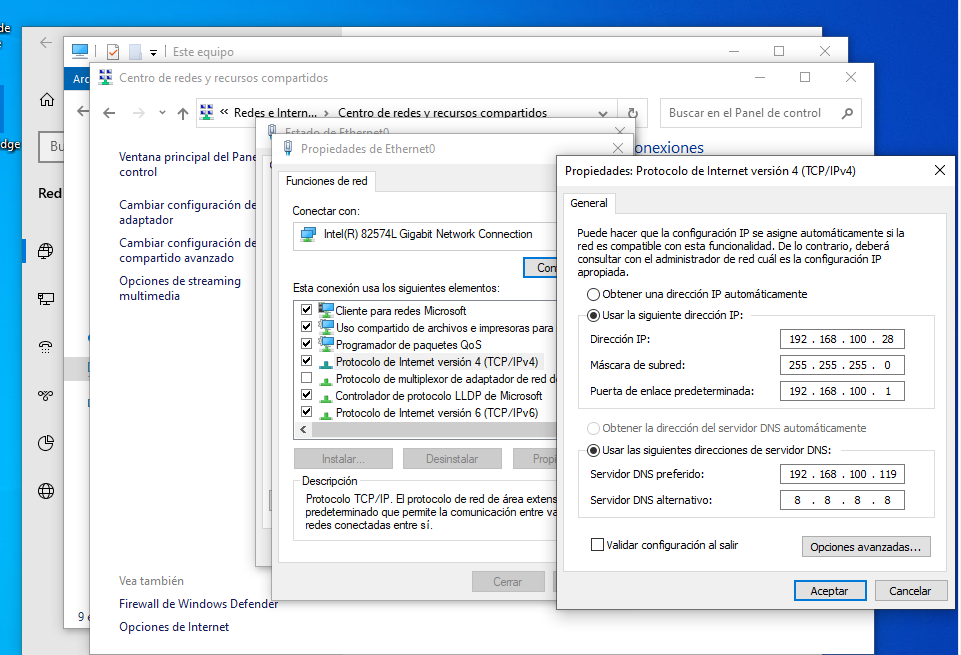
\includegraphics[width=0.8\textwidth]{config_red_win}
  \caption{Captura de administrador de dispositivos}\label{fig:confrwin}
\end{figure}

\end{itemize}

\newpage{}
\paragraph{SAMBA AD DC}\ \\Añadir cliente al demonio
\begin{itemize}
  \item Click derecho a equipo y \texttt{propiedades/configuracion avanzada/Nombre de equipo/ boton cambiar...}
        \begin{figure}[H]
          \centering
          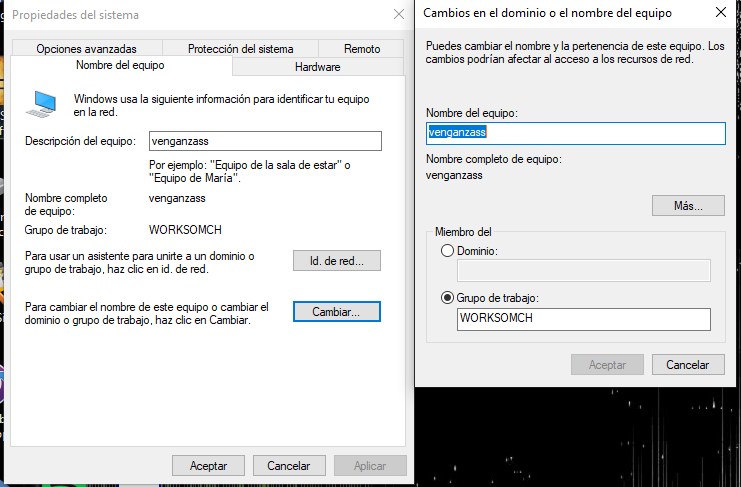
\includegraphics[width=0.8\textwidth]{config_cambiar}
          \caption{Configuracion del nombre del equipo}\label{fig:config_cambiar}
        \end{figure}
        \newpage{}

  \item En la seccion Miembro del seleccionar Dominio poner el dominio del servidor SAMBA que es \texttt{srv.nis}
        \begin{figure}[H]
          \centering
          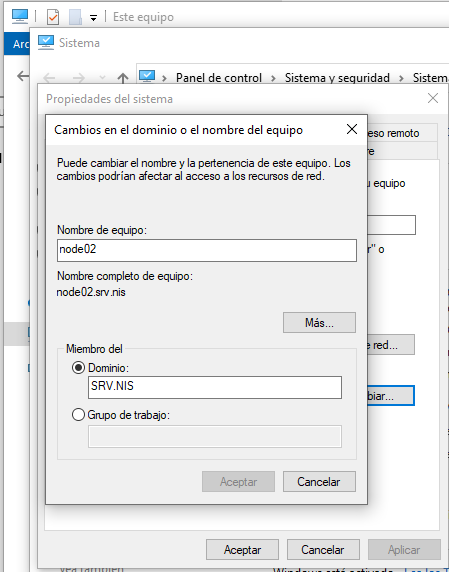
\includegraphics[width=0.8\textwidth]{config_cambiar_domi}
          \caption{Captura de asignacion de dominio}\label{fig:config_cambiar_domi}
        \end{figure}
        \newpage{}
  \item Si sale un dialogo de inicio de sesion usar el usuario ``Administrator''
        y poner la contraseña proporcionada en la configuracion
  \item Añadir el script \texttt{drive.bat} a la carpeta de programas
        de inicio para automontar la unidad \texttt{Z} al inicio de sesion de
        cada usuario.
        \begin{figure}[H]
          \centering
          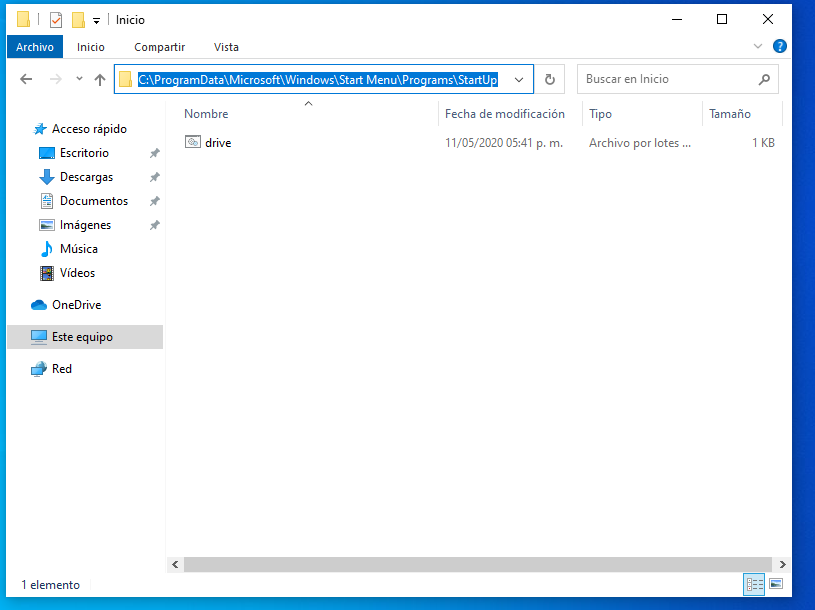
\includegraphics[width=0.8\textwidth]{menu_inicio}
          \caption{Captura de menu de inicio}\label{fig:menu_inicio}
        \end{figure}

        el contenido de este \texttt{drive.bat} es el siguiente:


        \begin{listing}[H]
\inputminted{bat}{../configs/drive.bat}
\caption{Contenido de drive.bat}
\label{listing:adduser.sh}
\end{listing}


  \item Para adaptar a caso de uso diferente
        modificar \texttt{SRV.NIS} por el nombre de dominio.
        correspondiente.
  \item Reiniciar equipo
        \newpage{}
  \item Si todo sale bien debe poder iniciar sesion con los
        usuarios creados en el servidor SAMBA
        \begin{figure}[H]
          \centering
          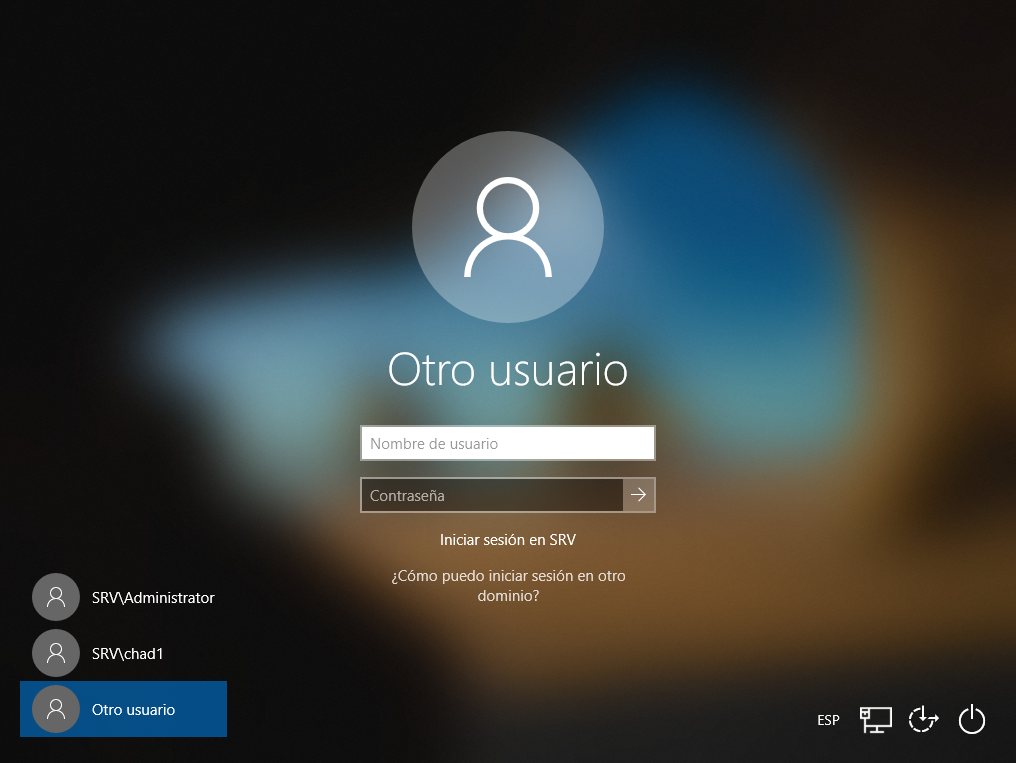
\includegraphics[width=0.8\textwidth]{inicio_sesion}
          \caption{Captura de inicio de sesion}\label{fig:inicio_sesion}
        \end{figure}
        \newpage{}
  \item La unidad Z con la carpeta home del usuario debe montarse al
        inicio de cada sesion
        \begin{figure}[H]
          \centering
          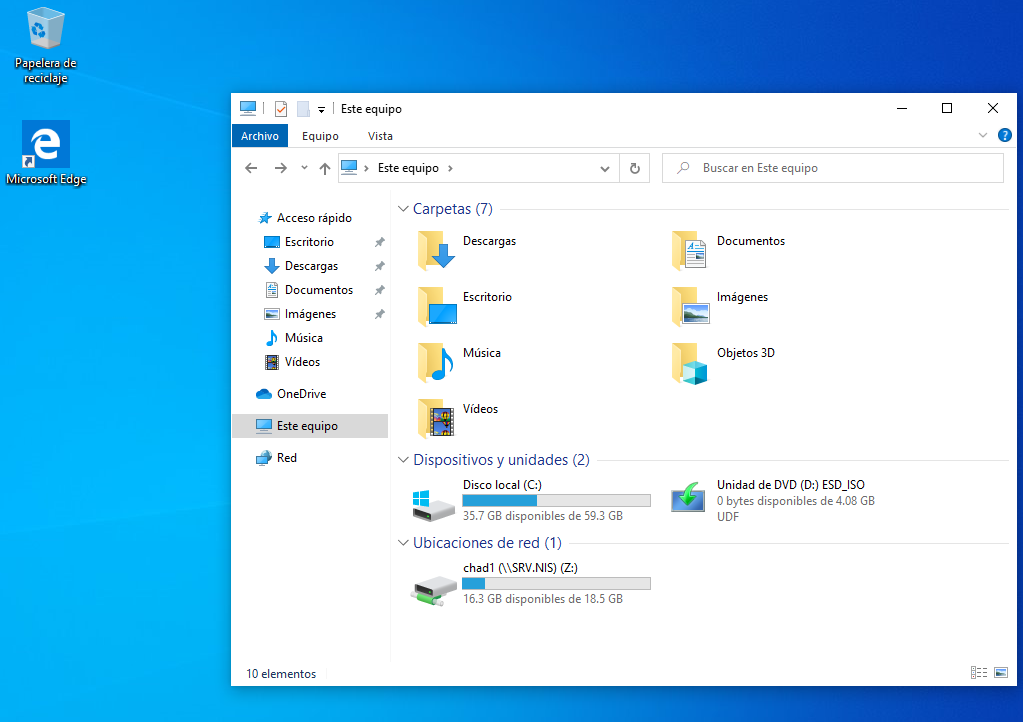
\includegraphics[width=0.8\textwidth]{samba_drive_z}
          \caption{Captura de inicio de sesion}\label{fig:samba_drive_z}
        \end{figure}

\end{itemize}


\end{document}
